% answers.tex —— 2004 年·普通高等学校招生考试·湖南卷·理科 · 参考答案与详细解析片段
% 由 tools/generate_projects.py 依来源总账自 2004/2004_数学真题_湖南理科_试题.md + 2004/2004_数学真题_湖南理科_解析正文.md + 2004/2004_数学真题_湖南理科_答案要点.md 生成，勿手改（改源 MD 后重跑）


\begin{gktip}
固定源 PDF 为印刷页码 174–175 的两页题面，不附官方答案。以下解析均依据固定源独立推导复算；各题配图在 LaTeX 工程中均以 TikZ 纯矢量重绘。第 3 题题面原卷印刷字符清晰为加号 $f(a+b)$，本库按真实字迹校订并给出完整证明。
\end{gktip}

\begin{answer}
\gksolhead{1}{}

\textbf{题目}：

复数 $\left(1 + \dfrac{1}{\mathrm{i}}\right)^4$ 的值是\mbox{（　　）}

\begin{gkopts}(4)
\task A．$4\mathrm{i}$
\task B．$-4\mathrm{i}$
\task C．$4$
\task D．$-4$
\end{gkopts}

\Needspace{4\baselineskip}
\textbf{解析}

\Needspace{5\baselineskip}
因为 $\dfrac{1}{\mathrm{i}} = -\mathrm{i}$，所以：
\nopagebreak[4]
\[
1 + \frac{1}{\mathrm{i}} = 1 - \mathrm{i}.
\]
\Needspace{5\baselineskip}
进而计算其平方：
\nopagebreak[4]
\[
(1 - \mathrm{i})^2 = 1 - 2\mathrm{i} + \mathrm{i}^2 = 1 - 2\mathrm{i} - 1 = -2\mathrm{i}.
\]
\Needspace{5\baselineskip}
因此：
\nopagebreak[4]
\[
\left(1 + \frac{1}{\mathrm{i}}\right)^4 = \left[(1 - \mathrm{i})^2\right]^2 = (-2\mathrm{i})^2 = 4\mathrm{i}^2 = -4.
\]

故选 D．

\gkanswer{答案：D}

\end{answer}
\begin{answer}
\gksolhead{2}{}

\textbf{题目}：

如果双曲线 $\dfrac{x^2}{13} - \dfrac{y^2}{12} = 1$ 上一点 $P$ 到右焦点的距离等于 $\sqrt{13}$，那么点 $P$ 到右准线的距离是\mbox{（　　）}

\begin{gkopts}(4)
\task A．$\dfrac{13}{5}$
\task B．$13$
\task C．$5$
\task D．$\dfrac{5}{13}$
\end{gkopts}

\Needspace{4\baselineskip}
\textbf{解析}

\Needspace{5\baselineskip}
由双曲线方程 $\dfrac{x^2}{13} - \dfrac{y^2}{12} = 1$ 可知：
\nopagebreak[4]
\[
a^2 = 13, \quad b^2 = 12, \quad c^2 = a^2 + b^2 = 13 + 12 = 25.
\]
\Needspace{5\baselineskip}
解得半焦距 $c = 5$，实半轴长 $a = \sqrt{13}$，故双曲线的离心率 $e$ 为：
\nopagebreak[4]
\[
e = \frac{c}{a} = \frac{5}{\sqrt{13}}.
\]
设点 $P$ 到右焦点 $F_2$ 的距离为 $|PF_2| = \sqrt{13}$，点 $P$ 到右准线的距离为 $d$．
\Needspace{5\baselineskip}
根据双曲线的第二定义，双曲线上任意一点到焦点的距离与它到相应准线的距离之比等于离心率 $e$：
\nopagebreak[4]
\[
\frac{|PF_2|}{d} = e \implies d = \frac{|PF_2|}{e}.
\]
\Needspace{5\baselineskip}
代入已知数值计算：
\nopagebreak[4]
\[
d = \frac{\sqrt{13}}{\dfrac{5}{\sqrt{13}}} = \frac{13}{5}.
\]

故选 A．

\gkanswer{答案：A}

\end{answer}
\begin{answer}
\gksolhead{3}{}

\textbf{题目}：

设 $f^{-1}(x)$ 是函数 $f(x) = \log_2(x + 1)$ 的反函数，若 $[1 + f^{-1}(a)][1 + f^{-1}(b)] = 8$，则 $f(a + b)$ 的值为\mbox{（　　）}

\begin{gkopts}(4)
\task A．$1$
\task B．$2$
\task C．$3$
\task D．$\log_2 3$
\end{gkopts}

\Needspace{4\baselineskip}
\textbf{解析}

函数 $f(x) = \log_2(x + 1)$（定义域为 $(-1, +\infty)$）．
\Needspace{5\baselineskip}
设 $y = \log_2(x + 1)$，则：
\nopagebreak[4]
\[
x + 1 = 2^y \implies x = 2^y - 1.
\]
\Needspace{5\baselineskip}
因此其反函数为：
\nopagebreak[4]
\[
f^{-1}(x) = 2^x - 1 \quad (x \in \mathbf{R}).
\]
\Needspace{5\baselineskip}
从而有：
\nopagebreak[4]
\[
1 + f^{-1}(a) = 1 + (2^a - 1) = 2^a, \quad 1 + f^{-1}(b) = 1 + (2^b - 1) = 2^b.
\]
\Needspace{5\baselineskip}
由已知条件 $[1 + f^{-1}(a)][1 + f^{-1}(b)] = 8$：
\nopagebreak[4]
\[
2^a \cdot 2^b = 8 \implies 2^{a+b} = 2^3 \implies a + b = 3.
\]
\Needspace{5\baselineskip}
原卷题面印刷清晰为加号 $f(a + b)$，代入得：
\nopagebreak[4]
\[
f(a + b) = f(3) = \log_2(3 + 1) = \log_2 4 = 2.
\]

故选 B．

\gkanswer{答案：B}

\end{answer}
\begin{answer}
\gksolhead{4}{}

\textbf{题目}：

把正方形 $ABCD$ 沿对角线 $AC$ 折起，当以 $A, B, C, D$ 四点为顶点的三棱锥体积最大时，直线 $BD$ 和平面 $ABC$ 所成的角的大小为\mbox{（　　）}

\begin{gkopts}(4)
\task A．$90^\circ$
\task B．$60^\circ$
\task C．$45^\circ$
\task D．$30^\circ$
\end{gkopts}

\Needspace{4\baselineskip}
\textbf{解析}

设正方形 $ABCD$ 的边长为 $1$，连接对角线 $AC$ 和 $BD$，设它们相交于点 $O$．
由正方形的几何性质可知，$BO \perp AC$，$DO \perp AC$，且 $BO = DO = \dfrac{\sqrt{2}}{2}$．
把正方形沿 $AC$ 折起后，在三棱锥 $D - ABC$ 中：
底面 $\triangle ABC$ 的面积为固定值 $S_{\triangle ABC} = \dfrac{1}{2} \times 1 \times 1 = \dfrac{1}{2}$．
三棱锥的体积 $V = \dfrac{1}{3} S_{\triangle ABC} \cdot h$，其中 $h$ 是点 $D$ 到平面 $ABC$ 的距离．
因为 $DO \perp AC$，所以点 $D$ 到平面 $ABC$ 的距离 $h \leqslant DO = \dfrac{\sqrt{2}}{2}$．
当且仅当 $DO \perp$ 平面 $ABC$（即平面 $DAC \perp$ 平面 $BAC$）时，$h$ 取得最大值 $\dfrac{\sqrt{2}}{2}$，此时三棱锥的体积最大．
在体积最大时，$DO \perp$ 平面 $ABC$，垂足为点 $O$．
因此直线 $BD$ 在平面 $ABC$ 内的射影为直线 $BO$．
所以直线 $BD$ 和平面 $ABC$ 所成的角即为 $\angle DBO$．
在 $\mathrm{Rt}\triangle DOB$ 中，$DO \perp BO$，且 $DO = BO = \dfrac{\sqrt{2}}{2}$．
故 $\triangle DOB$ 为等腰直角三角形，$\angle DBO = 45^\circ$．

故选 C．

\gkanswer{答案：C}

\end{answer}
\begin{answer}
\gksolhead{5}{}

\textbf{题目}：

某公司在甲、乙、丙、丁四个地区分别有 $150$ 个、$120$ 个、$180$ 个、$150$ 个销售点．公司为了调查产品销售的情况，需从这 $600$ 个销售点中抽取一个容量为 $100$ 的样本，记这项调查为①；在丙地区中有 $20$ 个特大型销售点，要从中抽取 $7$ 个调查其销售收入和售后服务情况，记这项调查为②．则完成①、②这两项调查宜采用的抽样方法依次是\mbox{（　　）}

\begin{gkopts}(2)
\task A．分层抽样，系统抽样法
\task B．分层抽样法，简单随机抽样法
\task C．系统抽样法，分层抽样法
\task D．简随机抽样法，分层抽样法
\end{gkopts}

\Needspace{4\baselineskip}
\textbf{解析}

对于调查①：
总体由甲、乙、丙、丁四个不同地区组成，各地区销售点数量存在明显差异且互不重叠．为了使样本能充分反映总体的分布结构，应当按照各地区的比例进行分层，因此宜采用分层抽样法．

对于调查②：
总体仅包含丙地区的 $20$ 个特大型销售点，样本容量为 $7$．由于总体容量较小，且每个销售点的性质均等、无明显层次差异，逐个不放回抽取最简便且随机性好，因此宜采用简单随机抽样法．

综上，完成①、②这两项调查宜采用的抽样方法依次是分层抽样法、简单随机抽样法．

故选 B．

\gkanswer{答案：B}

\end{answer}
\begin{answer}
\gksolhead{6}{}

\textbf{题目}：

设函数 $f(x) = \begin{cases} x^2 + bx + c, & x \leqslant 0, \\ 2, & x > 0. \end{cases}$ 若 $f(-4) = f(0)$，$f(-2) = -2$，则关于 $x$ 的方程 $f(x) = x$ 的解的个数为\mbox{（　　）}

\begin{gkopts}(4)
\task A．$1$
\task B．$2$
\task C．$3$
\task D．$4$
\end{gkopts}

\Needspace{4\baselineskip}
\textbf{解析}

当 $x \leqslant 0$ 时，$f(x) = x^2 + bx + c$．
\Needspace{5\baselineskip}
由已知 $f(-4) = f(0)$，得：
\nopagebreak[4]
\[
(-4)^2 - 4b + c = c \implies 16 - 4b = 0 \implies b = 4.
\]
\Needspace{5\baselineskip}
又 $f(-2) = -2$，代入得：
\nopagebreak[4]
\[
(-2)^2 + 4(-2) + c = -2 \implies 4 - 8 + c = -2 \implies c = 2.
\]
\Needspace{5\baselineskip}
因此分段函数为：
\nopagebreak[4]
\[
f(x) = \begin{cases} x^2 + 4x + 2, & x \leqslant 0, \\ 2, & x > 0. \end{cases}
\]
现在考查方程 $f(x) = x$ 的解：
\Needspace{5\baselineskip}
1. 当 $x \leqslant 0$ 时，方程为：
\nopagebreak[4]
\[
x^2 + 4x + 2 = x \implies x^2 + 3x + 2 = 0 \implies (x + 1)(x + 2) = 0.
\]
解得 $x_1 = -1$，$x_2 = -2$．因为 $-1 \leqslant 0$ 且 $-2 \leqslant 0$，两个解均符合条件，故在 $(-\infty, 0]$ 上有 $2$ 个解．
\Needspace{5\baselineskip}
2. 当 $x > 0$ 时，方程为：
\nopagebreak[4]
\[
2 = x \implies x = 2.
\]
因为 $2 > 0$，符合条件，故在 $(0, +\infty)$ 上有 $1$ 个解．

综上所述，方程 $f(x) = x$ 的解共有 $2 + 1 = 3$ 个．

故选 C．

\gkanswer{答案：C}

\end{answer}
\begin{answer}
\gksolhead{7}{}

\textbf{题目}：

设 $a > 0$，$b > 0$，则以下不等式中不恒成立的是\mbox{（　　）}

\begin{gkopts}(1)
\task A．$(a + b)\left(\dfrac{1}{a} + \dfrac{1}{b}\right) \geqslant 4$
\task B．$a^3 + b^3 \geqslant 2ab^2$
\task C．$a^2 + b^2 + 2 \geqslant 2a + 2b$
\task D．$\sqrt{|a - b|} \geqslant \sqrt{a} - \sqrt{b}$
\end{gkopts}

\Needspace{4\baselineskip}
\textbf{解析}

已知 $a > 0$，$b > 0$，逐项分析各不等式：

\Needspace{5\baselineskip}
对于 A 选项：
\nopagebreak[4]
\[
(a + b)\left(\frac{1}{a} + \frac{1}{b}\right) = 1 + \frac{b}{a} + \frac{a}{b} + 1 = 2 + \left(\frac{a}{b} + \frac{b}{a}\right).
\]
因为 $a > 0, b > 0$，由基本不等式 $\dfrac{a}{b} + \dfrac{b}{a} \geqslant 2$，故恒有 $(a + b)\left(\dfrac{1}{a} + \dfrac{1}{b}\right) \geqslant 4$，A 恒成立．

对于 B 选项：
考查作差：$a^3 + b^3 - 2ab^2$．
\Needspace{5\baselineskip}
取 $a = 2$，$b = 3$：
\nopagebreak[4]
\[
a^3 + b^3 = 2^3 + 3^3 = 8 + 27 = 35,
\]
\nopagebreak[4]
\[
2ab^2 = 2 \times 2 \times 3^2 = 36.
\]
此时 $35 < 36$，即 $a^3 + b^3 < 2ab^2$，故 B 选项不恒成立．

\Needspace{5\baselineskip}
对于 C 选项：
\nopagebreak[4]
\[
(a^2 + b^2 + 2) - (2a + 2b) = (a^2 - 2a + 1) + (b^2 - 2b + 1) = (a - 1)^2 + (b - 1)^2 \geqslant 0.
\]
故 $a^2 + b^2 + 2 \geqslant 2a + 2b$ 恒成立，C 恒成立．

对于 D 选项：
若 $a < b$，则 $\sqrt{a} - \sqrt{b} < 0$，而 $\sqrt{|a - b|} > 0$，不等式显然成立；
\Needspace{5\baselineskip}
若 $a \geqslant b > 0$，两边均为非负数，两边平方：
\nopagebreak[4]
\[
\left(\sqrt{|a - b|}\right)^2 = a - b,
\]
\nopagebreak[4]
\[
\left(\sqrt{a} - \sqrt{b}\right)^2 = a - 2\sqrt{ab} + b.
\]
\Needspace{5\baselineskip}
作差得：
\nopagebreak[4]
\[
(a - b) - (a - 2\sqrt{ab} + b) = 2\sqrt{ab} - 2b = 2\sqrt{b}(\sqrt{a} - \sqrt{b}) \geqslant 0.
\]
因此 $\sqrt{|a - b|} \geqslant \sqrt{a} - \sqrt{b}$ 恒成立，D 恒成立．

故选 B．

\gkanswer{答案：B}

\end{answer}
\begin{answer}
\gksolhead{8}{}

\textbf{题目}：

数列 $\{a_n\}$ 中，$a_1 = \dfrac{1}{5}$，$a_n + a_{n+1} = \dfrac{6}{5^{n+1}}$，$n \in \mathbf{N}^*$，则 $\lim\limits_{n \to \infty} (a_1 + a_2 + \cdots + a_n) =$\mbox{（　　）}

\begin{gkopts}(4)
\task A．$\dfrac{2}{5}$
\task B．$\dfrac{2}{7}$
\task C．$\dfrac{1}{4}$
\task D．$\dfrac{4}{25}$
\end{gkopts}

\Needspace{4\baselineskip}
\textbf{解析}

已知 $a_1 = \dfrac{1}{5}$，递推关系为 $a_n + a_{n+1} = \dfrac{6}{5^{n+1}}$ ($n \in \mathbf{N}^*$)．
\Needspace{5\baselineskip}
当 $n = 1$ 时：
\nopagebreak[4]
\[
a_1 + a_2 = \frac{6}{5^2} = \frac{6}{25} \implies a_2 = \frac{6}{25} - \frac{1}{5} = \frac{1}{25} = \left(\frac{1}{5}\right)^2.
\]
猜想数列通项为 $a_n = \left(\dfrac{1}{5}\right)^n$．
\Needspace{5\baselineskip}
检验递推关系：
\nopagebreak[4]
\[
a_n + a_{n+1} = \frac{1}{5^n} + \frac{1}{5^{n+1}} = \frac{5 + 1}{5^{n+1}} = \frac{6}{5^{n+1}}.
\]
满足已知递推公式．由数学归纳法可知，$a_n = \left(\dfrac{1}{5}\right)^n$ 对一切 $n \in \mathbf{N}^*$ 均成立．
因此数列 $\{a_n\}$ 是以 $a_1 = \dfrac{1}{5}$ 为首项、公比为 $q = \dfrac{1}{5}$ 的等比数列．
\Needspace{5\baselineskip}
由于 $|q| = \dfrac{1}{5} < 1$，其无穷项和存在，计算极限：
\nopagebreak[4]
\[
\lim_{n \to \infty} (a_1 + a_2 + \cdots + a_n) = \frac{a_1}{1 - q} = \frac{\dfrac{1}{5}}{1 - \dfrac{1}{5}} = \frac{\dfrac{1}{5}}{\dfrac{4}{5}} = \frac{1}{4}.
\]

故选 C．

\gkanswer{答案：C}

\end{answer}
\begin{answer}
\gksolhead{9}{}

\textbf{题目}：

设集合 $U = \{(x, y) \mid x \in \mathbf{R}, y \in \mathbf{R}\}$，$A = \{(x, y) \mid 2x - y + m > 0\}$，$B = \{(x, y) \mid x + y - n \leqslant 0\}$，那么点 $P(2, 3) \in A \cap (\complement_U B)$ 的充要条件是\mbox{（　　）}

\begin{gkopts}(4)
\task A．$m > -1, n < 5$
\task B．$m < -1, n < 5$
\task C．$m > -1, n > 5$
\task D．$m < -1, n > 5$
\end{gkopts}

\Needspace{4\baselineskip}
\textbf{解析}

全集 $U = \{(x, y) \mid x \in \mathbf{R}, y \in \mathbf{R}\}$．
集合 $A = \{(x, y) \mid 2x - y + m > 0\}$，集合 $B = \{(x, y) \mid x + y - n \leqslant 0\}$．
\Needspace{5\baselineskip}
点 $P(2, 3) \in A$ 的充要条件是将坐标代入 $A$ 的不等式成立：
\nopagebreak[4]
\[
2 \times 2 - 3 + m > 0 \implies 1 + m > 0 \implies m > -1.
\]
\Needspace{5\baselineskip}
根据补集定义，点 $P(2, 3) \in \complement_U B \iff P(2, 3) \notin B$，即点 $P$ 的坐标不满足 $x + y - n \leqslant 0$：
\nopagebreak[4]
\[
2 + 3 - n > 0 \implies 5 - n > 0 \implies n < 5.
\]
\Needspace{5\baselineskip}
因此，点 $P(2, 3) \in A \cap (\complement_U B)$ 的充要条件是：
\nopagebreak[4]
\[
m > -1 \text{ \text{且} } n < 5.
\]

故选 A．

\gkanswer{答案：A}

\end{answer}
\begin{answer}
\gksolhead{10}{}

\textbf{题目}：

从正方体的八个顶点中任取三个点为顶点作三角形，其中直角三角形的个数为\mbox{（　　）}

\begin{gkopts}(4)
\task A．$56$
\task B．$52$
\task C．$48$
\task D．$40$
\end{gkopts}

\Needspace{4\baselineskip}
\textbf{解析}

\Needspace{5\baselineskip}
正方体共有 $8$ 个顶点，从中任取 $3$ 个点作为顶点作三角形，总组合数为：
\nopagebreak[4]
\[
\mathrm{C}_8^3 = \frac{8 \times 7 \times 6}{3 \times 2 \times 1} = 56.
\]
在正方体中，由 $3$ 个顶点构成的三角形只有两类：直角三角形和正三角形．
正三角形的构成：
三边均为正方体的面对角线（边长为 $\sqrt{2}a$）．
正方体的 $8$ 个顶点中，每个顶角截出的截面对应一个正三角形（例如顶点 $A$ 对应 $\triangle A_1BD$），共有 $8$ 个这样的等边三角形．
容易验证，这 $8$ 个等边三角形的三边均相等，其内角均为 $60^\circ$，没有直角．
除这 $8$ 个等边三角形之外，其余任意由 $3$ 个顶点构成的三角形均含直角：
\begin{itemize}
\item 在同一表面内的三角形：每个正方形面内任取 $3$ 个顶点均为直角三角形，共有 $6 \times \mathrm{C}_4^3 = 6 \times 4 = 24$ 个；
\item 跨面的三角形：由一条面对角线与一条棱构成的三角形，例如面对角面内的三角形，共有 $24$ 个直角三角形．
\end{itemize}
\Needspace{5\baselineskip}
因此直角三角形的总个数为：
\nopagebreak[4]
\[
56 - 8 = 48.
\]

故选 C．

\gkanswer{答案：C}

\end{answer}
\begin{answer}
\gksolhead{11}{}

\textbf{题目}：

农民收入由工资性收入和其它收入两部分构成．2003 年某地区农民人均收入为 $3150$ 元（其中工资性收入为 $1800$ 元，其它收入为 $1350$ 元），预计该地区自 2004 年起的 $5$ 年内，农民的工资性收入将以每年 $6\%$ 的年增长率增长，其它收入每年增加 $160$ 元．根据以上数据，2008 年该地区农民人均收入介于\mbox{（　　）}

\begin{gkopts}(2)
\task A．$4200$ 元 $\sim 4400$ 元
\task B．$4400$ 元 $\sim 4600$ 元
\task C．$4600$ 元 $\sim 4800$ 元
\task D．$4800$ 元 $\sim 5000$ 元
\end{gkopts}

\Needspace{4\baselineskip}
\textbf{解析}

根据题意，2003 年农民人均收入为 $3150$ 元，其中工资性收入为 $1800$ 元，其它收入为 $1350$ 元．
从 2004 年起的 $5$ 年内，到 2008 年正好经历了 $5$ 年增长：
\Needspace{5\baselineskip}
1. 工资性收入每年以 $6\%$ 的增长率增长，2008 年的工资性收入为：
\nopagebreak[4]
\[
1800 \times (1 + 0.06)^5 = 1800 \times 1.06^5.
\]
\Needspace{5\baselineskip}
计算 $1.06^5$：
\nopagebreak[4]
\[
1.06^2 = 1.1236, \quad 1.06^4 = (1.1236)^2 \approx 1.262477, \quad 1.06^5 \approx 1.262477 \times 1.06 \approx 1.338226.
\]
\Needspace{5\baselineskip}
因此 2008 年工资性收入约为：
\nopagebreak[4]
\[
1800 \times 1.338226 \approx 2408.8 \text{ \text{元}}.
\]
\Needspace{5\baselineskip}
2. 其它收入每年增加 $160$ 元，5 年后增加 $5 \times 160 = 800$ 元，2008 年的其它收入为：
\nopagebreak[4]
\[
1350 + 800 = 2150 \text{ \text{元}}.
\]
\Needspace{5\baselineskip}
3. 2008 年农民人均总收入为：
\nopagebreak[4]
\[
2408.8 + 2150 = 4558.8 \text{ \text{元}}.
\]
数值介于 $4400$ 元 $\sim 4600$ 元之间．

故选 B．

\gkanswer{答案：B}

\end{answer}
\begin{answer}
\gksolhead{12}{}

\textbf{题目}：

设 $f(x)$、$g(x)$ 分别是定义在 $\mathbf{R}$ 上的奇函数和偶函数，当 $x < 0$ 时，$f'(x)g(x) + f(x)g'(x) > 0$，且 $g(-3) = 0$，则不等式 $f(x)g(x) < 0$ 的解集是\mbox{（　　）}

\begin{gkopts}(2)
\task A．$(-3, 0) \cup (3, +\infty)$
\task B．$(-3, 0) \cup (0, 3)$
\task C．$(-\infty, -3) \cup (3, +\infty)$
\task D．$(-\infty, -3) \cup (0, 3)$
\end{gkopts}

\Needspace{4\baselineskip}
\textbf{解析}

设辅助函数 $F(x) = f(x)g(x)$．
\Needspace{5\baselineskip}
已知 $f(x)$ 是定义在 $\mathbf{R}$ 上的奇函数，$g(x)$ 是定义在 $\mathbf{R}$ 上的偶函数，因此：
\nopagebreak[4]
\[
F(-x) = f(-x)g(-x) = [-f(x)]g(x) = -f(x)g(x) = -F(x).
\]
所以 $F(x)$ 是定义在 $\mathbf{R}$ 上的奇函数，且 $F(0) = 0$．
\Needspace{5\baselineskip}
对 $F(x)$ 求导：
\nopagebreak[4]
\[
F'(x) = f'(x)g(x) + f(x)g'(x).
\]
已知当 $x < 0$ 时，$f'(x)g(x) + f(x)g'(x) > 0$，即 $F'(x) > 0$．
因此 $F(x)$ 在 $(-\infty, 0)$ 上单调递增．
又已知 $g(-3) = 0$，所以 $F(-3) = f(-3)g(-3) = 0$．
结合单调性分析 $F(x)$ 在负半轴上的符号：
\begin{itemize}
\item 当 $x \in (-\infty, -3)$ 时，$F(x) < F(-3) = 0$；
\item 当 $x \in (-3, 0)$ 时，$F(x) > F(-3) = 0$．
\end{itemize}
利用奇函数的对称性：
$F(3) = -F(-3) = 0$．奇函数在关于原点对称的区间上具有相同的单调性，故 $F(x)$ 在 $(0, +\infty)$ 上也单调递增：
\begin{itemize}
\item 当 $x \in (0, 3)$ 时，$F(x) < F(3) = 0$；
\item 当 $x \in (3, +\infty)$ 时，$F(x) > F(3) = 0$．
\end{itemize}
\Needspace{5\baselineskip}
要求不等式 $f(x)g(x) < 0$，即 $F(x) < 0$ 的解集，即为：
\nopagebreak[4]
\[
(-\infty, -3) \cup (0, 3).
\]

故选 D．

\gkanswer{答案：D}

\end{answer}
\begin{answer}
\gksolhead{13}{}

\textbf{题目}：

已知向量 $\vec{a} = (\cos\theta, \sin\theta)$，向量 $\vec{b} = (\sqrt{3}, -1)$，则 $|2\vec{a} - \vec{b}|$ 的最大值是 $\underline{\hspace{2cm}}$．

\Needspace{4\baselineskip}
\textbf{解析}

\Needspace{5\baselineskip}
由已知 $\vec{a} = (\cos\theta, \sin\theta)$，得向量 $\vec{a}$ 的模为：
\nopagebreak[4]
\[
|\vec{a}| = \sqrt{\cos^2\theta + \sin^2\theta} = 1.
\]
故 $|2\vec{a}| = 2|\vec{a}| = 2$．
\Needspace{5\baselineskip}
向量 $\vec{b} = (\sqrt{3}, -1)$ 的模为：
\nopagebreak[4]
\[
|\vec{b}| = \sqrt{(\sqrt{3})^2 + (-1)^2} = \sqrt{3 + 1} = 2.
\]
\Needspace{5\baselineskip}
由三角形不等式：
\nopagebreak[4]
\[
|2\vec{a} - \vec{b}| \leqslant |2\vec{a}| + |\vec{b}| = 2 + 2 = 4.
\]
当 $2\vec{a}$ 与 $\vec{b}$ 反向共线时取得最大值 $4$．
故 $|2\vec{a} - \vec{b}|$ 的最大值是 $4$．

\gkanswer{答案：$4$}

\end{answer}
\begin{answer}
\gksolhead{14}{}

\textbf{题目}：

同时抛掷两枚相同的均匀硬币，随机变量 $\xi = 1$ 表示结果中有正面向上，$\xi = 0$ 表示结果中没有正面向上，则 $E\xi = \underline{\hspace{2cm}}$．

\Needspace{4\baselineskip}
\textbf{解析}

同时抛掷两枚相同的均匀硬币，所有等可能的基本事件总数为 $2 \times 2 = 4$ 种：
(正, 正)、(正, 反)、(反, 正)、(反, 反)．
随机变量 $\xi$ 的取值及其概率分布为：
\begin{itemize}
\item 当两枚硬币均为反面向上时，结果中没有正面向上，$\xi = 0$，其概率为：
\end{itemize}
\nopagebreak[4]
\[
P(\xi = 0) = \frac{1}{4}.
\]
\begin{itemize}
\item 其余情况均至少有一枚正面向上，$\xi = 1$，其概率为：
\end{itemize}
\nopagebreak[4]
\[
P(\xi = 1) = 1 - P(\xi = 0) = 1 - \frac{1}{4} = \frac{3}{4}.
\]
\Needspace{5\baselineskip}
根据数学期望的定义：
\nopagebreak[4]
\[
E\xi = 0 \times P(\xi = 0) + 1 \times P(\xi = 1) = 0 \times \frac{1}{4} + 1 \times \frac{3}{4} = \frac{3}{4}.
\]

\gkanswer{答案：$\dfrac{3}{4}$}

\end{answer}
\begin{answer}
\gksolhead{15}{}

\textbf{题目}：

若 $\left(x^3 + \dfrac{1}{x\sqrt{x}}\right)^n$ 的展开式中的常数项为 $84$，则 $n = \underline{\hspace{2cm}}$．

\Needspace{4\baselineskip}
\textbf{解析}

考查二项式 $\left(x^3 + \dfrac{1}{x\sqrt{x}}\right)^n$ 的展开式．
\Needspace{5\baselineskip}
因为 $\dfrac{1}{x\sqrt{x}} = x^{-\frac{3}{2}}$，所以二项展开式的通项公式为：
\nopagebreak[4]
\[
T_{r+1} = \mathrm{C}_n^r (x^3)^{n-r} (x^{-\frac{3}{2}})^r = \mathrm{C}_n^r x^{3n - 3r - \frac{3}{2}r} = \mathrm{C}_n^r x^{3n - \frac{9}{2}r}.
\]
\Needspace{5\baselineskip}
常数项要求 $x$ 的指数为 $0$：
\nopagebreak[4]
\[
3n - \frac{9}{2}r = 0 \implies 2n = 3r \implies r = \frac{2n}{3}.
\]
因为 $r$ 为整数，所以 $n$ 必须是 $3$ 的倍数，且 $0 \leqslant r \leqslant n$．
此时常数项的值为 $\mathrm{C}_n^r = 84$．
检验 $n$ 的取值：
\begin{itemize}
\item 若 $n = 6$，则 $r = 4$，$\mathrm{C}_6^4 = \mathrm{C}_6^2 = \dfrac{6 \times 5}{2} = 15 \neq 84$；
\item 若 $n = 9$，则 $r = 6$，$\mathrm{C}_9^6 = \mathrm{C}_9^3 = \dfrac{9 \times 8 \times 7}{3 \times 2 \times 1} = 84$．
\end{itemize}
完全符合题意，因此 $n = 9$．

\gkanswer{答案：$9$}

\end{answer}
\begin{answer}
\gksolhead{16}{}

\textbf{题目}：

设 $F$ 是椭圆 $\dfrac{x^2}{7} + \dfrac{y^2}{6} = 1$ 的右焦点，且椭圆上至少有 $21$ 个不同的点 $P_i$ ($i = 1, 2, 3, \cdots$)，使 $|FP_1|, |FP_2|, |FP_3|, \cdots$ 组成公差为 $d$ 的等差数列，则 $d$ 的取值范围为 $\underline{\hspace{2cm}}$．

\Needspace{4\baselineskip}
\textbf{解析}

椭圆方程为 $\dfrac{x^2}{7} + \dfrac{y^2}{6} = 1$，其中 $a^2 = 7, b^2 = 6$，半焦距 $c = \sqrt{a^2 - b^2} = \sqrt{7 - 6} = 1$．
右焦点为 $F(1, 0)$，离心率 $e = \dfrac{c}{a} = \dfrac{1}{\sqrt{7}}$．
\Needspace{5\baselineskip}
设椭圆上任意一点为 $P(x, y)$，由椭圆的焦半径公式：
\nopagebreak[4]
\[
|FP| = a - ex = \sqrt{7} - \frac{1}{\sqrt{7}}x.
\]
由于点 $P$ 在椭圆上，横坐标满足 $-\sqrt{7} \leqslant x \leqslant \sqrt{7}$：
\begin{itemize}
\item 当 $x = \sqrt{7}$（右顶点）时，$|FP|$ 取得最小值 $a - c = \sqrt{7} - 1$；
\item 当 $x = -\sqrt{7}$（左顶点）时，$|FP|$ 取得最大值 $a + c = \sqrt{7} + 1$．
\end{itemize}
\Needspace{5\baselineskip}
因此焦半径 $|FP|$ 的取值范围为闭区间 $[\sqrt{7} - 1, \sqrt{7} + 1]$，其区间长度为：
\nopagebreak[4]
\[
(\sqrt{7} + 1) - (\sqrt{7} - 1) = 2.
\]
由椭圆的对称性：
\begin{itemize}
\item 当焦半径取两个端点值 $\sqrt{7} - 1$ 或 $\sqrt{7} + 1$ 时，椭圆上各仅有 $1$ 个点（即左、右顶点）；
\item 当焦半径取开区间 $(\sqrt{7} - 1, \sqrt{7} + 1)$ 内的任意一个数值时，由 $x = \dfrac{a - |FP|}{e} \in (-a, a)$ 确定唯一的横坐标 $x$，对应的纵坐标有两个 $y = \pm \sqrt{6\left(1 - \dfrac{x^2}{7}\right)}$，即椭圆上恰好对应上下对称的 $2$ 个不同的点．
\end{itemize}
要使椭圆上至少有 $21$ 个不同的点 $P_i$ 的焦半径构成公差为 $d > 0$ 的等差数列：
设等差数列各项取出的互不相同的焦半径值为 $r_1 < r_2 < \cdots < r_k$．
\Needspace{5\baselineskip}
由于每个焦半径值最多提供 $2$ 个点，若数列的不同焦半径取值个数 $k \leqslant 11$，则椭圆上能产生的不同点数至多为：
\nopagebreak[4]
\[
1 + 2 \times 9 + 1 = 20 < 21.
\]
因此，要得到至少 $21$ 个不同的点，等差数列中必须至少包含 $12$ 个不同的焦半径值（$12$ 个值最多可对应 $20 + 2 = 22$ 个点，满足不低于 $21$ 个的要求）．
这 $12$ 个互不相同的项全部落在区间 $[\sqrt{7} - 1, \sqrt{7} + 1]$ 内，其首末跨度为 $11d$．
\Needspace{5\baselineskip}
因此必须满足：
\nopagebreak[4]
\[
11d \leqslant (\sqrt{7} + 1) - (\sqrt{7} - 1) = 2 \implies d \leqslant \frac{2}{11}.
\]
又由公差 $d > 0$，故 $d$ 的取值范围为 $\left(0, \dfrac{2}{11}\right]$．

\gkanswer{答案：$\left(0, \dfrac{2}{11}\right]$}

\end{answer}
\begin{answer}
\gksolhead{17}{}

\textbf{题目}：

（本小题满分 12 分）

已知 $\sin\left(\dfrac{\pi}{4} + 2\alpha\right) \cdot \sin\left(\dfrac{\pi}{4} - 2\alpha\right) = \dfrac{1}{4}$，$\alpha \in \left(\dfrac{\pi}{4}, \dfrac{\pi}{2}\right)$，求 $2\sin^2\alpha + \tan\alpha - \cot\alpha - 1$ 的值．

\Needspace{4\baselineskip}
\textbf{解析}

\Needspace{5\baselineskip}
已知三角条件式为：
\nopagebreak[4]
\[
\sin\left(\frac{\pi}{4} + 2\alpha\right) \cdot \sin\left(\frac{\pi}{4} - 2\alpha\right) = \frac{1}{4}.
\]
\Needspace{5\baselineskip}
利用三角积化和差公式：
\nopagebreak[4]
\[
\sin A \sin B = -\frac{1}{2}[\cos(A + B) - \cos(A - B)].
\]
\Needspace{5\baselineskip}
这里 $A + B = \dfrac{\pi}{2}$，$A - B = 4\alpha$，所以：
\nopagebreak[4]
\[
-\frac{1}{2}\left[\cos\frac{\pi}{2} - \cos 4\alpha\right] = \frac{1}{4} \implies \frac{1}{2}\cos 4\alpha = \frac{1}{4} \implies \cos 4\alpha = \frac{1}{2}.
\]
已知 $\alpha \in \left(\dfrac{\pi}{4}, \dfrac{\pi}{2}\right)$，故 $2\alpha \in \left(\dfrac{\pi}{2}, \pi\right)$，$4\alpha \in (\pi, 2\pi)$．
\Needspace{5\baselineskip}
在此区间内，满足 $\cos 4\alpha = \dfrac{1}{2}$ 的角为：
\nopagebreak[4]
\[
4\alpha = 2\pi - \frac{\pi}{3} = \frac{5\pi}{3} \implies 2\alpha = \frac{5\pi}{6}.
\]
\Needspace{5\baselineskip}
因此：
\nopagebreak[4]
\[
\cos 2\alpha = \cos\frac{5\pi}{6} = -\frac{\sqrt{3}}{2}, \quad \sin 2\alpha = \sin\frac{5\pi}{6} = \frac{1}{2}.
\]
\Needspace{5\baselineskip}
现在化简所求目标式：
\nopagebreak[4]
\[
2\sin^2\alpha + \tan\alpha - \cot\alpha - 1 = (2\sin^2\alpha - 1) + (\tan\alpha - \cot\alpha).
\]
由倍角公式，$2\sin^2\alpha - 1 = -\cos 2\alpha$．
\Needspace{5\baselineskip}
将第二项化简：
\nopagebreak[4]
\[
\tan\alpha - \cot\alpha = \frac{\sin\alpha}{\cos\alpha} - \frac{\cos\alpha}{\sin\alpha} = \frac{\sin^2\alpha - \cos^2\alpha}{\sin\alpha\cos\alpha} = \frac{-\cos 2\alpha}{\dfrac{1}{2}\sin 2\alpha} = -\frac{2\cos 2\alpha}{\sin 2\alpha}.
\]
\Needspace{5\baselineskip}
代入合并得：
\nopagebreak[4]
\[
-\cos 2\alpha - \frac{2\cos 2\alpha}{\sin 2\alpha} = -\cos 2\alpha\left(1 + \frac{2}{\sin 2\alpha}\right).
\]
\Needspace{5\baselineskip}
将 $\cos 2\alpha = -\dfrac{\sqrt{3}}{2}$ 与 $\sin 2\alpha = \dfrac{1}{2}$ 代入计算：
\nopagebreak[4]
\[
-\left(-\frac{\sqrt{3}}{2}\right)\left(1 + \frac{2}{\dfrac{1}{2}}\right) = \frac{\sqrt{3}}{2}(1 + 4) = \frac{5\sqrt{3}}{2}.
\]

\gkanswer{答案：$\dfrac{5\sqrt{3}}{2}$}

\end{answer}
\begin{answer}
\gksolhead{18}{}

\textbf{题目}：

（本小题满分 12 分）

如图，在底面是菱形的四棱锥 $P - ABCD$ 中，$\angle ABC = 60^\circ$，$PA = AC = a$，$PB = PD = \sqrt{2}a$，点 $E$ 在 $PD$ 上，且 $PE : ED = 2 : 1$．
\nopagebreak[4]
\begin{center}% Source-faithful schematic draft: 2004 Hunan Science Q18, PDF p.1 (printed p.174).
% Source ID: src-9f80071b553ab4b942482c92509eda24ffc4990bd51cd38172372a29634438da
% Source SHA-256: 47ba4497f88a0667fcfd694f4b8a9a37e7b1d3f098a0ad26b0529b990194e2c7
\begin{tikzpicture}[line width=0.6pt,scale=1.1,every node/.style={inner sep=1.5pt}]
  % Coordinates of pyramid P-ABCD with rhombus base ABCD
  % A is behind, PA is perpendicular to base ABCD
  \coordinate (A) at (0, 0);
  \coordinate (B) at (-1.8, -0.9);
  \coordinate (C) at (0.2, -1.5);
  \coordinate (D) at (2.0, 0);
  \coordinate (P) at (0, 2.5);
  \coordinate (E) at ($(P)!0.6667!(D)$);

  % Dashed interior lines
  \draw[dashed, line width=0.5pt] (P) -- (A);
  \draw[dashed, line width=0.5pt] (A) -- (B);
  \draw[dashed, line width=0.5pt] (A) -- (D);
  \draw[dashed, line width=0.5pt] (A) -- (C);
  \draw[dashed, line width=0.5pt] (A) -- (E);

  % Solid exterior edges and section lines
  \draw (P) -- (B);
  \draw (P) -- (D);
  \draw (B) -- (C);
  \draw (C) -- (D);
  \draw (E) -- (C);

  % Vertex labels faithful to original layout
  \node[above] at (P) {$P$};
  \node[above left] at (A) {$A$};
  \node[below left] at (B) {$B$};
  \node[below] at (C) {$C$};
  \node[right] at (D) {$D$};
  \node[above right] at (E) {$E$};
\end{tikzpicture}
\end{center}
\nopagebreak[4]
(1) 证明：$PA \perp$ 平面 $ABCD$；

(2) 求以 $AC$ 为棱，$EAC$ 与 $DAC$ 为面的二面角 $\theta$ 的大小；

(3) 在棱 $PC$ 上是否存在一点 $F$，使 $BF \parallel$ 平面 $AEC$？证明你的结论．

\Needspace{4\baselineskip}
\textbf{解析}
\nopagebreak[4]
\begin{center}% Source-faithful schematic draft: 2004 Hunan Science Q18, PDF p.1 (printed p.174).
% Source ID: src-9f80071b553ab4b942482c92509eda24ffc4990bd51cd38172372a29634438da
% Source SHA-256: 47ba4497f88a0667fcfd694f4b8a9a37e7b1d3f098a0ad26b0529b990194e2c7
\begin{tikzpicture}[line width=0.6pt,scale=1.1,every node/.style={inner sep=1.5pt}]
  % Coordinates of pyramid P-ABCD with rhombus base ABCD
  % A is behind, PA is perpendicular to base ABCD
  \coordinate (A) at (0, 0);
  \coordinate (B) at (-1.8, -0.9);
  \coordinate (C) at (0.2, -1.5);
  \coordinate (D) at (2.0, 0);
  \coordinate (P) at (0, 2.5);
  \coordinate (E) at ($(P)!0.6667!(D)$);

  % Dashed interior lines
  \draw[dashed, line width=0.5pt] (P) -- (A);
  \draw[dashed, line width=0.5pt] (A) -- (B);
  \draw[dashed, line width=0.5pt] (A) -- (D);
  \draw[dashed, line width=0.5pt] (A) -- (C);
  \draw[dashed, line width=0.5pt] (A) -- (E);

  % Solid exterior edges and section lines
  \draw (P) -- (B);
  \draw (P) -- (D);
  \draw (B) -- (C);
  \draw (C) -- (D);
  \draw (E) -- (C);

  % Vertex labels faithful to original layout
  \node[above] at (P) {$P$};
  \node[above left] at (A) {$A$};
  \node[below left] at (B) {$B$};
  \node[below] at (C) {$C$};
  \node[right] at (D) {$D$};
  \node[above right] at (E) {$E$};
\end{tikzpicture}
\end{center}
\nopagebreak[4]
\textbf{(1)} 证明：
四棱锥 $P - ABCD$ 的底面 $ABCD$ 为菱形，已知 $\angle ABC = 60^\circ$．
在 $\triangle ABC$ 中，$AB = BC$，且 $\angle ABC = 60^\circ$，所以 $\triangle ABC$ 为等边三角形，从而 $AB = BC = AC = a$．
又菱形的四边长均相等，所以 $AD = a$．
\Needspace{5\baselineskip}
在 $\triangle PAB$ 中，已知 $PA = a$，$AB = a$，$PB = \sqrt{2}a$，满足：
\nopagebreak[4]
\[
PA^2 + AB^2 = a^2 + a^2 = 2a^2 = PB^2.
\]
由勾股定理逆定理可知，$PA \perp AB$．
\Needspace{5\baselineskip}
同理在 $\triangle PAD$ 中，已知 $PA = a$，$AD = a$，$PD = \sqrt{2}a$，满足：
\nopagebreak[4]
\[
PA^2 + AD^2 = a^2 + a^2 = 2a^2 = PD^2.
\]
由勾股定理逆定理可知，$PA \perp AD$．
因为 $AB \cap AD = A$，且 $AB, AD \subset$ 平面 $ABCD$．
所以 $PA \perp$ 平面 $ABCD$．

\textbf{(2)} 解：
因为底面 $ABCD$ 是菱形，对角线互相垂直，设 $AC \cap BD = O$，则 $DO \perp AC$．
在等边 $\triangle ABC$ 中，$AC = a$，$OA = OC = \dfrac{a}{2}$，菱形边长为 $a$．
由勾股定理，$DO = \sqrt{AD^2 - OA^2} = \sqrt{a^2 - \left(\dfrac{a}{2}\right)^2} = \dfrac{\sqrt{3}}{2}a$．
已知点 $E$ 在棱 $PD$ 上，且 $PE : ED = 2 : 1$，故 $ED = \dfrac{1}{3}PD$．
在平面 $PAD$ 内，过点 $E$ 作 $EH \perp AD$ 于点 $H$．
\Needspace{5\baselineskip}
因为 $PA \perp AD$，所以 $EH \parallel PA$，且：
\nopagebreak[4]
\[
\frac{EH}{PA} = \frac{ED}{PD} = \frac{1}{3} \implies EH = \frac{1}{3}PA = \frac{a}{3}, \quad DH = \frac{1}{3}AD = \frac{a}{3}.
\]
因为 $PA \perp$ 平面 $ABCD$，所以 $EH \perp$ 平面 $ABCD$．
在平面 $ABCD$ 内，过点 $H$ 作 $HM \perp AC$ 于点 $M$．
\Needspace{5\baselineskip}
由于 $DO \perp AC$，故 $HM \parallel DO$．在 $\triangle ADO$ 中，由相似三角形性质：
\nopagebreak[4]
\[
\frac{HM}{DO} = \frac{AH}{AD} = \frac{a - \dfrac{a}{3}}{a} = \frac{2}{3} \implies HM = \frac{2}{3} DO = \frac{2}{3} \times \frac{\sqrt{3}}{2}a = \frac{\sqrt{3}}{3}a.
\]
连接 $EM$．因为 $EH \perp$ 平面 $ABCD$，$HM \perp AC$ 于点 $M$，$HM \subset$ 平面 $ABCD$，由三垂线定理可得 $EM \perp AC$．
因此 $\angle EMH$ 即为以 $AC$ 为棱，$EAC$ 与 $DAC$ 为面的二面角 $\theta$ 的平面角．
\Needspace{5\baselineskip}
在 $\mathrm{Rt}\triangle EHM$ 中：
\nopagebreak[4]
\[
\tan\theta = \frac{EH}{HM} = \frac{\dfrac{a}{3}}{\dfrac{\sqrt{3}}{3}a} = \frac{1}{\sqrt{3}} = \frac{\sqrt{3}}{3}.
\]
因为 $\theta \in \left(0, \dfrac{\pi}{2}\right)$，所以二面角 $\theta$ 的大小为 $30^\circ$（或 $\dfrac{\pi}{6}$）．

\textbf{(3)} 解：
在棱 $PC$ 上存在一点 $F$，使得 $BF \parallel$ 平面 $AEC$，该点 $F$ 为棱 $PC$ 的中点．证明如下：
在平面 $PBD$ 中，连接 $BD$ 交 $AC$ 于点 $O$．由菱形对角线互相平分可知，点 $O$ 为 $BD$ 的中点．
连接 $EO$，在平面 $PBD$ 内延长 $EO$，与 $PB$ 的延长线相交于点 $G$．
\Needspace{5\baselineskip}
在 $\triangle PBD$ 中，割线 $GEO$ 截边 $PD, BD$ 及 $PB$ 的延长线，由梅涅劳斯定理：
\nopagebreak[4]
\[
\frac{PE}{ED} \cdot \frac{DO}{OB} \cdot \frac{BG}{GP} = 1.
\]
\Needspace{5\baselineskip}
已知 $\dfrac{PE}{ED} = \dfrac{2}{1}$，且点 $O$ 为 $BD$ 中点即 $\dfrac{DO}{OB} = 1$，代入得：
\nopagebreak[4]
\[
\frac{2}{1} \cdot 1 \cdot \frac{BG}{GP} = 1 \implies \frac{GP}{BG} = 2.
\]
因此点 $B$ 为线段 $PG$ 的中点．
在 $\triangle PGC$ 中，因为点 $B$ 为 $PG$ 的中点，取点 $F$ 为 $PC$ 的中点，连接 $BF$．
\Needspace{5\baselineskip}
则 $BF$ 是 $\triangle PGC$ 的中位线，因此：
\nopagebreak[4]
\[
BF \parallel GC.
\]
因为点 $G$ 落在直线 $EO$ 的延长线上，而直线 $EO \subset$ 平面 $AEC$，所以点 $G \in$ 平面 $AEC$．
又点 $C \in$ 平面 $AEC$，所以直线 $GC \subset$ 平面 $AEC$．
而直线 $BF \not\subset$ 平面 $AEC$．
\Needspace{5\baselineskip}
根据直线与平面平行的判定定理，可知：
\nopagebreak[4]
\[
BF \parallel \text{\text{平面} } AEC.
\]
所以，在棱 $PC$ 上存在一点 $F$（为棱 $PC$ 的中点），使得 $BF \parallel$ 平面 $AEC$．

\gkanswer{答案（1）：见解析版}

\gkanswer{答案（2）：$30^\circ$（或 $\dfrac{\pi}{6}$）。}

\gkanswer{答案（3）：在棱 $PC$ 上存在点 $F$，当点 $F$ 为棱 $PC$ 的中点时，$BF \parallel$ 平面 $AEC$，证明见解析。}

\end{answer}
\begin{answer}
\gksolhead{19}{}

\textbf{题目}：

（本小题满分 12 分）

甲、乙、丙三台机床各自独立地加工同一种零件，已知甲机床加工的零件是一等品而乙机床加工的零件不是一等品的概率为 $\dfrac{1}{4}$，乙机床加工的零件是一等品而丙机床加工的零件不是一等品的概率为 $\dfrac{1}{12}$，甲、丙两台机床加工的零件都是一等品的概率为 $\dfrac{2}{9}$．

(1) 分别求甲、乙、丙三台机床各自加工零件是一等品的概率；

(2) 从甲、乙、丙加工的零件中各取一个检验，求至少有一个一等品的概率．

\Needspace{4\baselineskip}
\textbf{解析}

\textbf{(1)} 解：
设甲、乙、丙三台机床各自加工零件是一等品的概率分别为 $P_1, P_2, P_3$．
\Needspace{5\baselineskip}
由于三台机床独立工作，根据独立事件的概率乘法公式，由已知条件建立方程组：
\nopagebreak[4]
\[
\begin{cases}
P_1(1 - P_2) = \dfrac{1}{4}, & \text{(i)} \\[2mm]
P_2(1 - P_3) = \dfrac{1}{12}, & \text{(ii)} \\[2mm]
P_1 P_3 = \dfrac{2}{9}. & \text{(iii)}
\end{cases}
\]
\Needspace{5\baselineskip}
由式 (iii) 可解得：
\nopagebreak[4]
\[
P_3 = \frac{2}{9P_1}.
\]
\Needspace{5\baselineskip}
将其代入式 (ii)：
\nopagebreak[4]
\[
P_2\left(1 - \frac{2}{9P_1}\right) = \frac{1}{12} \implies P_2 \cdot \frac{9P_1 - 2}{9P_1} = \frac{1}{12} \implies P_2 = \frac{3P_1}{4(9P_1 - 2)}.
\]
\Needspace{5\baselineskip}
由式 (i) 可得：
\nopagebreak[4]
\[
1 - P_2 = \frac{1}{4P_1} \implies P_2 = 1 - \frac{1}{4P_1} = \frac{4P_1 - 1}{4P_1}.
\]
\Needspace{5\baselineskip}
将两个关于 $P_2$ 的表达式联立：
\nopagebreak[4]
\[
\frac{4P_1 - 1}{4P_1} = \frac{3P_1}{4(9P_1 - 2)}.
\]
\Needspace{5\baselineskip}
两边同乘以 $4P_1(9P_1 - 2)$ 整理得：
\nopagebreak[4]
\[
(4P_1 - 1)(9P_1 - 2) = 3P_1^2 \implies 36P_1^2 - 17P_1 + 2 = 3P_1^2 \implies 33P_1^2 - 17P_1 + 2 = 0.
\]
\Needspace{5\baselineskip}
因式分解得：
\nopagebreak[4]
\[
(3P_1 - 1)(11P_1 - 2) = 0.
\]
\Needspace{5\baselineskip}
解得：
\nopagebreak[4]
\[
P_1 = \frac{1}{3} \quad \text{\text{或}} \quad P_1 = \frac{2}{11}.
\]
\begin{itemize}
\item 若 $P_1 = \dfrac{2}{11}$，则 $P_3 = \dfrac{2}{9P_1} = \dfrac{2}{9 \times \dfrac{2}{11}} = \dfrac{11}{9} > 1$，与概率值 $0 \leqslant P_3 \leqslant 1$ 矛盾，舍去；
\item 若 $P_1 = \dfrac{1}{3}$，则：
\end{itemize}
\nopagebreak[4]
\[
P_3 = \frac{2}{9 \times \dfrac{1}{3}} = \frac{2}{3}, \quad P_2 = 1 - \frac{1}{4 \times \dfrac{1}{3}} = 1 - \frac{3}{4} = \frac{1}{4}.
\]
均满足概率在 $[0, 1]$ 范围内的要求．
因此，甲、乙、丙三台机床各自加工零件是一等品的概率分别为 $\dfrac{1}{3}$，$\dfrac{1}{4}$，$\dfrac{2}{3}$．

\textbf{(2)} 解：
设事件 $A$ 为“从甲、乙、丙加工的零件中各取一个检验，至少有一个一等品”．
其对立事件 $\overline{A}$ 为“取出的三个零件都不是一等品”．
由于三台机床加工相互独立，各个零件不是一等品的概率分别为 $1 - P_1$、$1 - P_2$、$1 - P_3$．
\Needspace{5\baselineskip}
因此：
\nopagebreak[4]
\[
P(\overline{A}) = (1 - P_1)(1 - P_2)(1 - P_3) = \left(1 - \frac{1}{3}\right)\left(1 - \frac{1}{4}\right)\left(1 - \frac{2}{3}\right) = \frac{2}{3} \times \frac{3}{4} \times \frac{1}{3} = \frac{1}{6}.
\]
\Needspace{5\baselineskip}
所以至少有一个一等品的概率为：
\nopagebreak[4]
\[
P(A) = 1 - P(\overline{A}) = 1 - \frac{1}{6} = \frac{5}{6}.
\]

\gkanswer{答案（1）：甲、乙、丙加工零件是一等品的概率分别为 $\dfrac{1}{3}$，$\dfrac{1}{4}$，$\dfrac{2}{3}$。}

\gkanswer{答案（2）：$\dfrac{5}{6}$。}

\end{answer}
\begin{answer}
\gksolhead{20}{}

\textbf{题目}：

（本小题满分 12 分）

已知函数 $f(x) = x^2 \mathrm{e}^{ax}$，其中 $a \leqslant 0$，$\mathrm{e}$ 为自然对数的底数．

(1) 讨论函数 $f(x)$ 的单调性；

(2) 求函数 $f(x)$ 在区间 $[0, 1]$ 上的最大值．

\Needspace{4\baselineskip}
\textbf{解析}

\textbf{(1)} 解：
\Needspace{5\baselineskip}
对函数 $f(x) = x^2 \mathrm{e}^{ax}$ 求导：
\nopagebreak[4]
\[
f'(x) = 2x \mathrm{e}^{ax} + x^2 (a\mathrm{e}^{ax}) = x(ax + 2)\mathrm{e}^{ax}.
\]
因为对任意 $x \in \mathbf{R}$ 恒有 $\mathrm{e}^{ax} > 0$，所以 $f'(x)$ 的符号由二次因式 $x(ax + 2)$ 决定．
分两种情况讨论单调性：
1. 当 $a = 0$ 时，$f(x) = x^2$，$f'(x) = 2x$：
\begin{itemize}
\item 当 $x \in (-\infty, 0)$ 时，$f'(x) < 0$；当 $x \in (0, +\infty)$ 时，$f'(x) > 0$．
\item 故 $f(x)$ 的单调递减区间为 $(-\infty, 0]$，单调递增区间为 $[0, +\infty)$．
\end{itemize}
2. 当 $a < 0$ 时，令 $f'(x) = 0$，解得两个互异根：$x_1 = 0$，$x_2 = -\dfrac{2}{a} > 0$．
\begin{itemize}
\item 当 $x \in (-\infty, 0)$ 时，$x < 0$ 且 $ax + 2 > 2 > 0$，故 $f'(x) < 0$；
\item 当 $x \in \left(0, -\dfrac{2}{a}\right)$ 时，$x > 0$ 且 $ax + 2 > 0$，故 $f'(x) > 0$；
\item 当 $x \in \left(-\dfrac{2}{a}, +\infty\right)$ 时，$x > 0$ 且 $ax + 2 < 0$，故 $f'(x) < 0$．
\item 故 $f(x)$ 的单调递减区间为 $(-\infty, 0]$ 和 $\left[-\dfrac{2}{a}, +\infty\right)$，单调递增区间为 $\left[0, -\dfrac{2}{a}\right]$．
\end{itemize}

\textbf{(2)} 解：
考查函数 $f(x)$ 在闭区间 $[0, 1]$ 上的最大值：
\begin{itemize}
\item 若 $a = 0$：
\end{itemize}
\Needspace{5\baselineskip}
  由 (1) 可知 $f(x)$ 在 $[0, +\infty)$ 上单调递增，故在 $[0, 1]$ 上单调递增，其最大值为：
\nopagebreak[4]
\[
f(1) = 1^2 \cdot \mathrm{e}^{0 \times 1} = 1.
\]
\begin{itemize}
\item 若 $a < 0$：
\end{itemize}
  极值点为 $x = -\dfrac{2}{a} > 0$．
  ① 当 $-\dfrac{2}{a} \geqslant 1$，即 $-2 \leqslant a < 0$ 时：
  区间 $[0, 1] \subseteq \left[0, -\dfrac{2}{a}\right]$，此时 $f(x)$ 在 $[0, 1]$ 上单调递增．
\Needspace{5\baselineskip}
  故最大值在右端点 $x = 1$ 处取得：
\nopagebreak[4]
\[
f(1) = 1^2 \cdot \mathrm{e}^{a \times 1} = \mathrm{e}^a.
\]
  注意当 $a = 0$ 时 $\mathrm{e}^0 = 1$，两者形式一致，可统一合并为：当 $-2 \leqslant a \leqslant 0$ 时，最大值为 $\mathrm{e}^a$．
  ② 当 $-\dfrac{2}{a} < 1$，即 $a < -2$ 时：
  极值点 $-\dfrac{2}{a} \in (0, 1)$．
  $f(x)$ 在 $\left[0, -\dfrac{2}{a}\right]$ 上单调递增，在 $\left[-\dfrac{2}{a}, 1\right]$ 上单调递减．
\Needspace{5\baselineskip}
  故最大值在极大值点 $x = -\dfrac{2}{a}$ 处取得：
\nopagebreak[4]
\[
f\left(-\frac{2}{a}\right) = \left(-\frac{2}{a}\right)^2 \mathrm{e}^{a\left(-\frac{2}{a}\right)} = \frac{4}{a^2} \mathrm{e}^{-2} = \frac{4}{a^2 \mathrm{e}^2}.
\]
综上所述：
\begin{itemize}
\item 当 $-2 \leqslant a \leqslant 0$ 时，$f(x)$ 在区间 $[0, 1]$ 上的最大值为 $\mathrm{e}^a$；
\item 当 $a < -2$ 时，$f(x)$ 在区间 $[0, 1]$ 上的最大值为 $\dfrac{4}{a^2 \mathrm{e}^2}$．
\end{itemize}

\gkanswer{答案（1）：当 $a = 0$ 时，单调递减区间为 $(-\infty, 0]$，单调递增区间为 $[0, +\infty)$；当 $a < 0$ 时，单调递减区间为 $(-\infty, 0]$ 和 $\left[-\dfrac{2}{a}, +\infty\right)$，单调递增区间为 $\left[0, -\dfrac{2}{a}\right]$。}

\gkanswer{答案（2）：当 $-2 \leqslant a \leqslant 0$ 时，最大值为 $\mathrm{e}^a$；当 $a < -2$ 时，最大值为 $\dfrac{4}{a^2 \mathrm{e}^2}$。}

\end{answer}
\begin{answer}
\gksolhead{21}{}

\textbf{题目}：

（本小题满分 13 分）

如图，过抛物线 $x^2 = 4y$ 的对称轴上任一点 $P(0, m)$ ($m > 0$) 作直线与抛物线交于 $A, B$ 两点，点 $Q$ 是点 $P$ 关于原点的对称点．
\nopagebreak[4]
\begin{center}% Source-faithful schematic draft: 2004 Hunan Science Q21, PDF p.2 (printed p.175).
% Source ID: src-9f80071b553ab4b942482c92509eda24ffc4990bd51cd38172372a29634438da
% Source SHA-256: 47ba4497f88a0667fcfd694f4b8a9a37e7b1d3f098a0ad26b0529b990194e2c7
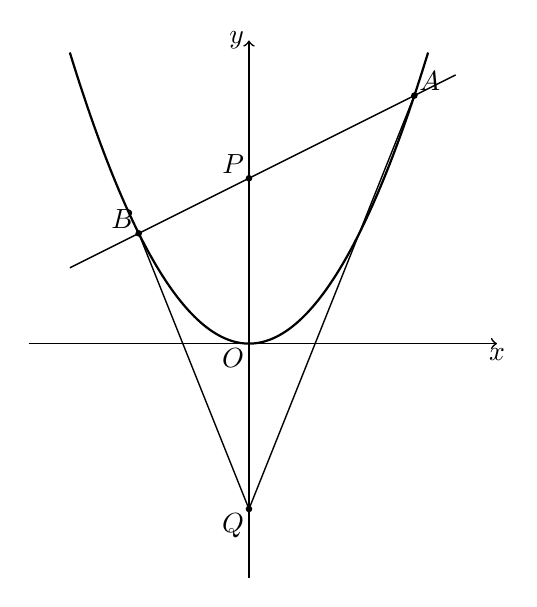
\begin{tikzpicture}[line width=0.6pt,scale=0.35,every node/.style={inner sep=1.5pt}]
  % Axes
  \draw[->] (-8, 0) -- (9, 0) node[below] {$x$};
  \draw[->] (0, -8.5) -- (0, 11) node[left] {$y$};
  \node[below left] at (0, 0) {$O$};

  % Parabola x^2 = 4y => y = x^2 / 4
  \draw[thick,domain=-6.5:6.5,samples=60,smooth] plot (\x, {0.25*\x*\x});

  % Points P(0, 6) and Q(0, -6)
  \coordinate (P) at (0, 6);
  \coordinate (Q) at (0, -6);
  \fill (P) circle (0.12) node[above left] {$P$};
  \fill (Q) circle (0.12) node[below left] {$Q$};

  % Points A(6, 9) and B(-4, 4) on parabola and line y = 0.5x + 6
  \coordinate (A) at (6, 9);
  \coordinate (B) at (-4, 4);
  \fill (A) circle (0.12) node[above right] {$A$};
  \fill (B) circle (0.12) node[above left] {$B$};

  % Secant line AB passing through P
  \draw[line width=0.55pt] (-6.5, 2.75) -- (7.5, 9.75);

  % Lines QA and QB
  \draw[line width=0.5pt] (Q) -- (A);
  \draw[line width=0.5pt] (Q) -- (B);
\end{tikzpicture}
\end{center}
\nopagebreak[4]
(1) 设点 $P$ 分有向线段 $\vec{AB}$ 所成的比为 $\lambda$，证明：$\vec{QP} \perp (\vec{QA} - \lambda\vec{QB})$；

(2) 设直线 $AB$ 的方程是 $x - 2y + 12 = 0$，过 $A, B$ 两点的圆 $C$ 与抛物线在点 $A$ 处有共同的切线，求圆 $C$ 的方程．

\Needspace{4\baselineskip}
\textbf{解析}
\nopagebreak[4]
\begin{center}% Source-faithful schematic draft: 2004 Hunan Science Q21, PDF p.2 (printed p.175).
% Source ID: src-9f80071b553ab4b942482c92509eda24ffc4990bd51cd38172372a29634438da
% Source SHA-256: 47ba4497f88a0667fcfd694f4b8a9a37e7b1d3f098a0ad26b0529b990194e2c7
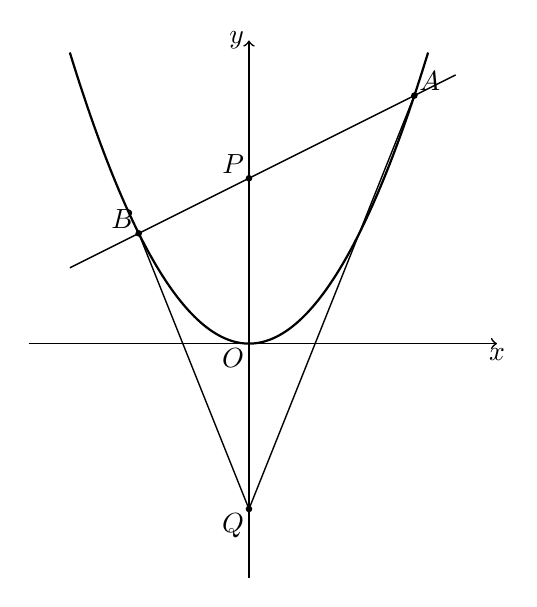
\begin{tikzpicture}[line width=0.6pt,scale=0.35,every node/.style={inner sep=1.5pt}]
  % Axes
  \draw[->] (-8, 0) -- (9, 0) node[below] {$x$};
  \draw[->] (0, -8.5) -- (0, 11) node[left] {$y$};
  \node[below left] at (0, 0) {$O$};

  % Parabola x^2 = 4y => y = x^2 / 4
  \draw[thick,domain=-6.5:6.5,samples=60,smooth] plot (\x, {0.25*\x*\x});

  % Points P(0, 6) and Q(0, -6)
  \coordinate (P) at (0, 6);
  \coordinate (Q) at (0, -6);
  \fill (P) circle (0.12) node[above left] {$P$};
  \fill (Q) circle (0.12) node[below left] {$Q$};

  % Points A(6, 9) and B(-4, 4) on parabola and line y = 0.5x + 6
  \coordinate (A) at (6, 9);
  \coordinate (B) at (-4, 4);
  \fill (A) circle (0.12) node[above right] {$A$};
  \fill (B) circle (0.12) node[above left] {$B$};

  % Secant line AB passing through P
  \draw[line width=0.55pt] (-6.5, 2.75) -- (7.5, 9.75);

  % Lines QA and QB
  \draw[line width=0.5pt] (Q) -- (A);
  \draw[line width=0.5pt] (Q) -- (B);
\end{tikzpicture}
\end{center}
\nopagebreak[4]
\textbf{(1)} 证明：
点 $P(0, m)$ ($m > 0$) 在抛物线对称轴（$y$ 轴）上，点 $Q$ 是点 $P$ 关于原点的对称点，故点 $Q$ 的坐标为 $(0, -m)$．
从而向量 $\vec{QP} = (0 - 0, m - (-m)) = (0, 2m)$．
设直线 $AB$ 的斜率为 $k$，则其方程为 $y = kx + m$．
\Needspace{5\baselineskip}
联立直线方程与抛物线方程：
\nopagebreak[4]
\[
\begin{cases}
y = kx + m, \\
x^2 = 4y.
\end{cases}
\]
\Needspace{5\baselineskip}
消去 $y$ 得关于 $x$ 的一元二次方程：
\nopagebreak[4]
\[
x^2 - 4kx - 4m = 0.
\]
\Needspace{5\baselineskip}
设点 $A(x_1, y_1)$，点 $B(x_2, y_2)$，由韦达定理：
\nopagebreak[4]
\[
x_1 + x_2 = 4k, \quad x_1 x_2 = -4m.
\]
因为点 $P$ 分有向线段 $\vec{AB}$ 所成的比为 $\lambda$，即 $\vec{AP} = \lambda\vec{PB}$．
\Needspace{5\baselineskip}
在 $x$ 轴上的投影坐标关系为：
\nopagebreak[4]
\[
0 - x_1 = \lambda(x_2 - 0) \implies -x_1 = \lambda x_2 \implies \lambda = -\frac{x_1}{x_2}.
\]
由 $x_1 x_2 = -4m < 0$ 可知 $x_1, x_2$ 异号，故 $\lambda > 0$．
又 $\vec{QA} = (x_1, y_1 + m)$，$\vec{QB} = (x_2, y_2 + m)$，
\Needspace{5\baselineskip}
因此向量 $\vec{QA} - \lambda\vec{QB}$ 的坐标为：
\nopagebreak[4]
\[
\vec{QA} - \lambda\vec{QB} = \Big(x_1 - \lambda x_2, \, (y_1 + m) - \lambda(y_2 + m)\Big).
\]
\Needspace{5\baselineskip}
考查其纵坐标：
\nopagebreak[4]
\[
(y_1 + m) - \lambda(y_2 + m) = y_1 - \lambda y_2 + (1 - \lambda)m.
\]
\Needspace{5\baselineskip}
由于点 $A, B$ 在抛物线上，$y_1 = \dfrac{x_1^2}{4}$，$y_2 = \dfrac{x_2^2}{4}$，将 $\lambda = -\dfrac{x_1}{x_2}$ 代入：
\nopagebreak[4]
\[
y_1 - \lambda y_2 = \frac{x_1^2}{4} - \left(-\frac{x_1}{x_2}\right)\frac{x_2^2}{4} = \frac{x_1^2 + x_1 x_2}{4}.
\]
\Needspace{5\baselineskip}
又由 $x_1 x_2 = -4m$，得 $m = -\dfrac{x_1 x_2}{4}$，代入计算：
\nopagebreak[4]
\[
(1 - \lambda)m = \left(1 + \frac{x_1}{x_2}\right)\left(-\frac{x_1 x_2}{4}\right) = \frac{x_1 + x_2}{x_2}\left(-\frac{x_1 x_2}{4}\right) = -\frac{x_1(x_1 + x_2)}{4} = -\frac{x_1^2 + x_1 x_2}{4}.
\]
\Needspace{5\baselineskip}
因此：
\nopagebreak[4]
\[
(y_1 + m) - \lambda(y_2 + m) = \frac{x_1^2 + x_1 x_2}{4} - \frac{x_1^2 + x_1 x_2}{4} = 0.
\]
所以向量 $\vec{QA} - \lambda\vec{QB} = (x_1 - \lambda x_2, 0)$ 的纵坐标恒为 $0$．
\Needspace{5\baselineskip}
于是：
\nopagebreak[4]
\[
\vec{QP} \cdot (\vec{QA} - \lambda\vec{QB}) = 0 \times (x_1 - \lambda x_2) + 2m \times 0 = 0.
\]
因此 $\vec{QP} \perp (\vec{QA} - \lambda\vec{QB})$ 得证．

\textbf{(2)} 解：
直线 $AB$ 的方程为 $x - 2y + 12 = 0$，即 $y = \dfrac{1}{2}x + 6$．
\Needspace{5\baselineskip}
将其与抛物线方程 $x^2 = 4y$ 联立：
\nopagebreak[4]
\[
x^2 = 4\left(\frac{1}{2}x + 6\right) = 2x + 24 \implies x^2 - 2x - 24 = 0.
\]
解得 $(x - 6)(x + 4) = 0 \implies x_1 = 6, x_2 = -4$．
由图形布局，点 $A$ 在第一象限，点 $B$ 在第二象限：
\begin{itemize}
\item 当 $x = 6$ 时，$y = \dfrac{6^2}{4} = 9$，点 $A(6, 9)$；
\item 当 $x = -4$ 时，$y = \dfrac{(-4)^2}{4} = 4$，点 $B(-4, 4)$．
\end{itemize}
对抛物线 $y = \dfrac{x^2}{4}$ 求导，得切线斜率函数 $y' = \dfrac{x}{2}$．
\Needspace{5\baselineskip}
在点 $A(6, 9)$ 处，切线斜率为：
\nopagebreak[4]
\[
k_{\text{\text{切}}} = \frac{6}{2} = 3.
\]
因为圆 $C$ 与抛物线在点 $A$ 处有共同的切线，所以圆心 $C(x_0, y_0)$ 必定落在点 $A$ 处的法线上．
\Needspace{5\baselineskip}
过点 $A$ 的法线斜率为 $k_{\text{\text{法}}} = -\dfrac{1}{k_{\text{\text{切}}}} = -\dfrac{1}{3}$，法线方程为：
\nopagebreak[4]
\[
y - 9 = -\frac{1}{3}(x - 6) \implies x + 3y - 33 = 0.
\]
\Needspace{5\baselineskip}
故圆心坐标满足方程：
\nopagebreak[4]
\[
x_0 + 3y_0 - 33 = 0. \quad \text{(i)}
\]
又圆 $C$ 经过 $A(6, 9)$ 和 $B(-4, 4)$ 两点，圆心 $C$ 必在线段 $AB$ 的垂直平分线上．
\Needspace{5\baselineskip}
线段 $AB$ 的中点坐标为：
\nopagebreak[4]
\[
\left(\frac{6 + (-4)}{2}, \frac{9 + 4}{2}\right) = \left(1, \frac{13}{2}\right).
\]
线段 $AB$ 的斜率为 $\dfrac{9 - 4}{6 - (-4)} = \dfrac{5}{10} = \dfrac{1}{2}$，其垂直平分线的斜率为 $-2$．
\Needspace{5\baselineskip}
垂直平分线方程为：
\nopagebreak[4]
\[
y - \frac{13}{2} = -2(x - 1) \implies 2x + y - \frac{17}{2} = 0 \implies 4x + 2y - 17 = 0.
\]
\Needspace{5\baselineskip}
故圆心坐标满足方程：
\nopagebreak[4]
\[
4x_0 + 2y_0 - 17 = 0. \quad \text{(ii)}
\]
联立方程 (i) 与 (ii)：
\Needspace{5\baselineskip}
由 (i) 得 $x_0 = 33 - 3y_0$，代入 (ii) 得：
\nopagebreak[4]
\[
4(33 - 3y_0) + 2y_0 - 17 = 0 \implies 132 - 12y_0 + 2y_0 - 17 = 0 \implies 10y_0 = 115 \implies y_0 = \frac{23}{2}.
\]
\Needspace{5\baselineskip}
代回求 $x_0$：
\nopagebreak[4]
\[
x_0 = 33 - 3 \times \frac{23}{2} = 33 - \frac{69}{2} = -\frac{3}{2}.
\]
因此圆心坐标为 $C\left(-\dfrac{3}{2}, \dfrac{23}{2}\right)$．
\Needspace{5\baselineskip}
圆的半径平方为：
\nopagebreak[4]
\[
R^2 = |CA|^2 = \left(6 - \left(-\frac{3}{2}\right)\right)^2 + \left(9 - \frac{23}{2}\right)^2 = \left(\frac{15}{2}\right)^2 + \left(-\frac{5}{2}\right)^2 = \frac{225 + 25}{4} = \frac{250}{4} = \frac{125}{2}.
\]
\Needspace{5\baselineskip}
所以圆 $C$ 的方程为：
\nopagebreak[4]
\[
\left(x + \frac{3}{2}\right)^2 + \left(y - \frac{23}{2}\right)^2 = \frac{125}{2}.
\]
（展开式为 $x^2 + y^2 + 3x - 23y + 72 = 0$）．

\gkanswer{答案（1）：见解析版}

\gkanswer{答案（2）：$\left(x + \dfrac{3}{2}\right)^2 + \left(y - \dfrac{23}{2}\right)^2 = \dfrac{125}{2}$（或 $x^2 + y^2 + 3x - 23y + 72 = 0$）。}

\end{answer}
\begin{answer}
\gksolhead{22}{}

\textbf{题目}：

（本小题满分 13 分）

如图，直线 $l_1: y = kx + 1 - k$ $\left(k \neq 0, k \neq \pm \dfrac{1}{2}\right)$ 与 $l_2: y = \dfrac{1}{2}x + \dfrac{1}{2}$ 相交于点 $P$．直线 $l_1$ 与 $x$ 轴交于点 $P_1$，过点 $P_1$ 作 $x$ 轴的垂线交直线 $l_2$ 于点 $Q_1$，过点 $Q_1$ 作 $y$ 轴的垂线交直线 $l_1$ 于点 $P_2$，过点 $P_2$ 作 $x$ 轴的垂线交直线 $l_2$ 于点 $Q_2$，$\cdots$，这样一直作下去，可得到一系列点 $P_1, Q_1, P_2, Q_2, \cdots$．点 $P_n$ ($n = 1, 2, \cdots$) 的横坐标构成数列 $\{x_n\}$．
\nopagebreak[4]
\begin{center}% Source-faithful schematic draft: 2004 Hunan Science Q22, PDF p.2 (printed p.175).
% Source ID: src-9f80071b553ab4b942482c92509eda24ffc4990bd51cd38172372a29634438da
% Source SHA-256: 47ba4497f88a0667fcfd694f4b8a9a37e7b1d3f098a0ad26b0529b990194e2c7
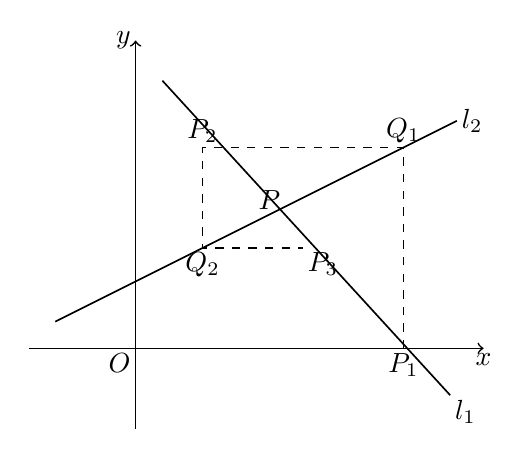
\begin{tikzpicture}[line width=0.6pt,scale=1.7,every node/.style={inner sep=1.5pt}]
  % Axes
  \draw[->] (-0.8, 0) -- (2.6, 0) node[below] {$x$};
  \draw[->] (0, -0.6) -- (0, 2.3) node[left] {$y$};
  \node[below left] at (0, 0) {$O$};

  % Coordinates based on k = -1:
  % P(1, 1), l1: y = -x + 2, l2: y = 0.5x + 0.5
  \coordinate (P) at (1, 1);
  \coordinate (P1) at (2, 0);
  \coordinate (Q1) at (2, 1.5);
  \coordinate (P2) at (0.5, 1.5);
  \coordinate (Q2) at (0.5, 0.75);
  \coordinate (P3) at (1.25, 0.75);

  % Line l1
  \draw[line width=0.6pt] (0.2, 2.0) -- (2.35, -0.35) node[below right] {$l_1$};

  % Line l2
  \draw[line width=0.6pt] (-0.6, 0.2) -- (2.4, 1.7) node[right] {$l_2$};

  % Dashed staircase lines
  \draw[dashed, line width=0.5pt] (P1) -- (Q1) -- (P2) -- (Q2) -- (P3);

  % Labels
  \node[above] at (P) {$P$};
  \node[below] at (P1) {$P_1$};
  \node[above] at (Q1) {$Q_1$};
  \node[above] at (P2) {$P_2$};
  \node[below] at (Q2) {$Q_2$};
  \node[below right] at (P3) {$P_3$};
\end{tikzpicture}
\end{center}
\nopagebreak[4]
(1) 证明：$x_{n+1} - 1 = \dfrac{1}{2k}(x_n - 1)$，$n \in \mathbf{N}^*$；

(2) 求数列 $\{x_n\}$ 的通项公式；

(3) 比较 $2|PP_n|^2$ 与 $4k^2|PP_1|^2 + 5$ 的大小．

\Needspace{4\baselineskip}
\textbf{解析}
\nopagebreak[4]
\begin{center}% Source-faithful schematic draft: 2004 Hunan Science Q22, PDF p.2 (printed p.175).
% Source ID: src-9f80071b553ab4b942482c92509eda24ffc4990bd51cd38172372a29634438da
% Source SHA-256: 47ba4497f88a0667fcfd694f4b8a9a37e7b1d3f098a0ad26b0529b990194e2c7
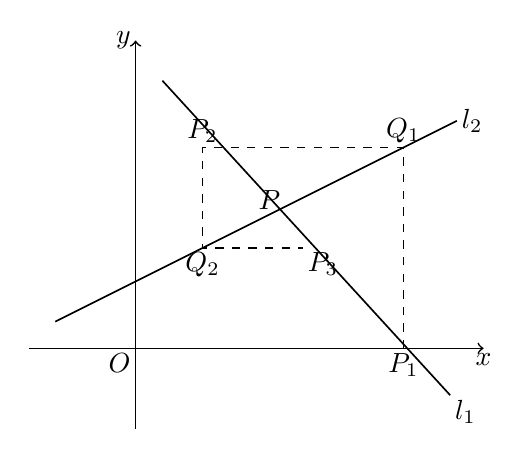
\begin{tikzpicture}[line width=0.6pt,scale=1.7,every node/.style={inner sep=1.5pt}]
  % Axes
  \draw[->] (-0.8, 0) -- (2.6, 0) node[below] {$x$};
  \draw[->] (0, -0.6) -- (0, 2.3) node[left] {$y$};
  \node[below left] at (0, 0) {$O$};

  % Coordinates based on k = -1:
  % P(1, 1), l1: y = -x + 2, l2: y = 0.5x + 0.5
  \coordinate (P) at (1, 1);
  \coordinate (P1) at (2, 0);
  \coordinate (Q1) at (2, 1.5);
  \coordinate (P2) at (0.5, 1.5);
  \coordinate (Q2) at (0.5, 0.75);
  \coordinate (P3) at (1.25, 0.75);

  % Line l1
  \draw[line width=0.6pt] (0.2, 2.0) -- (2.35, -0.35) node[below right] {$l_1$};

  % Line l2
  \draw[line width=0.6pt] (-0.6, 0.2) -- (2.4, 1.7) node[right] {$l_2$};

  % Dashed staircase lines
  \draw[dashed, line width=0.5pt] (P1) -- (Q1) -- (P2) -- (Q2) -- (P3);

  % Labels
  \node[above] at (P) {$P$};
  \node[below] at (P1) {$P_1$};
  \node[above] at (Q1) {$Q_1$};
  \node[above] at (P2) {$P_2$};
  \node[below] at (Q2) {$Q_2$};
  \node[below right] at (P3) {$P_3$};
\end{tikzpicture}
\end{center}
\nopagebreak[4]
\Needspace{5\baselineskip}
首先联立直线 $l_1$ 与 $l_2$ 的方程求交点 $P$：
\nopagebreak[4]
\[
kx + 1 - k = \frac{1}{2}x + \frac{1}{2} \implies \left(k - \frac{1}{2}\right)x = k - \frac{1}{2}.
\]
已知 $k \neq \dfrac{1}{2}$，解得 $x = 1$．代入求得 $y = \dfrac{1}{2}(1) + \dfrac{1}{2} = 1$．
故两直线交于定点 $P(1, 1)$．直线方程可写为点斜式 $l_1: y - 1 = k(x - 1)$，$l_2: y - 1 = \dfrac{1}{2}(x - 1)$．

\textbf{(1)} 证明：
\Needspace{5\baselineskip}
由题意，点 $P_n$ 在直线 $l_1$ 上，设其坐标为 $(x_n, y_{P_n})$，则满足：
\nopagebreak[4]
\[
y_{P_n} = k(x_n - 1) + 1.
\]
过点 $P_n$ 作 $x$ 轴的垂线交直线 $l_2$ 于点 $Q_n$，则点 $Q_n$ 的横坐标与 $P_n$ 相同为 $x_n$．
\Needspace{5\baselineskip}
因为点 $Q_n$ 在直线 $l_2$ 上，其纵坐标为：
\nopagebreak[4]
\[
y_{Q_n} = \frac{1}{2}(x_n - 1) + 1.
\]
\Needspace{5\baselineskip}
过点 $Q_n$ 作 $y$ 轴的垂线交直线 $l_1$ 于点 $P_{n+1}$，则点 $P_{n+1}$ 的纵坐标与 $Q_n$ 相同：
\nopagebreak[4]
\[
y_{P_{n+1}} = y_{Q_n} = \frac{1}{2}(x_n - 1) + 1.
\]
\Needspace{5\baselineskip}
又因为点 $P_{n+1}$ 在直线 $l_1$ 上，其纵坐标亦满足：
\nopagebreak[4]
\[
y_{P_{n+1}} = k(x_{n+1} - 1) + 1.
\]
\Needspace{5\baselineskip}
因此：
\nopagebreak[4]
\[
k(x_{n+1} - 1) + 1 = \frac{1}{2}(x_n - 1) + 1 \implies k(x_{n+1} - 1) = \frac{1}{2}(x_n - 1).
\]
\Needspace{5\baselineskip}
因为 $k \neq 0$，两边同除以 $k$ 即可得到：
\nopagebreak[4]
\[
x_{n+1} - 1 = \frac{1}{2k}(x_n - 1), \quad n \in \mathbf{N}^*.
\]

\textbf{(2)} 解：
\Needspace{5\baselineskip}
点 $P_1$ 是直线 $l_1$ 与 $x$ 轴的交点，令 $y = 0$：
\nopagebreak[4]
\[
k(x_1 - 1) + 1 = 0 \implies k(x_1 - 1) = -1 \implies x_1 - 1 = -\frac{1}{k}.
\]
由 (1) 可知，数列 $\{x_n - 1\}$ 是以 $x_1 - 1 = -\dfrac{1}{k}$ 为首项、公比 $q = \dfrac{1}{2k}$ 的等比数列．
\Needspace{5\baselineskip}
由等比数列通项公式：
\nopagebreak[4]
\[
x_n - 1 = (x_1 - 1) q^{n-1} = \left(-\frac{1}{k}\right)\left(\frac{1}{2k}\right)^{n-1} = -2\left(\frac{1}{2k}\right)^n.
\]
\Needspace{5\baselineskip}
因此数列 $\{x_n\}$ 的通项公式为：
\nopagebreak[4]
\[
x_n = 1 - 2\left(\frac{1}{2k}\right)^n.
\]

\textbf{(3)} 解：
因为点 $P(1, 1)$，点 $P_n(x_n, y_{P_n})$ 在直线 $l_1$ 上，且 $y_{P_n} - 1 = k(x_n - 1)$．
\Needspace{5\baselineskip}
由两点间距离公式：
\nopagebreak[4]
\[
|PP_n|^2 = (x_n - 1)^2 + (y_{P_n} - 1)^2 = (x_n - 1)^2 + k^2(x_n - 1)^2 = (1 + k^2)(x_n - 1)^2.
\]
\Needspace{5\baselineskip}
特别地，当 $n = 1$ 时，$(x_1 - 1)^2 = \left(-\dfrac{1}{k}\right)^2 = \dfrac{1}{k^2}$，故：
\nopagebreak[4]
\[
|PP_1|^2 = \frac{1 + k^2}{k^2}.
\]
\Needspace{5\baselineskip}
计算式子 $4k^2|PP_1|^2 + 5$：
\nopagebreak[4]
\[
4k^2|PP_1|^2 + 5 = 4k^2 \cdot \frac{1 + k^2}{k^2} + 5 = 4(1 + k^2) + 5 = 4k^2 + 9.
\]
\Needspace{5\baselineskip}
将 (2) 中的 $(x_n - 1)^2 = 4\left(\dfrac{1}{2k}\right)^{2n} = \dfrac{4}{(4k^2)^n}$ 代入 $2|PP_n|^2$：
\nopagebreak[4]
\[
2|PP_n|^2 = 2(1 + k^2) \cdot \frac{4}{(4k^2)^n} = \frac{8(1 + k^2)}{(4k^2)^n}.
\]
记 $u = 4k^2$．因为 $k \neq 0$ 且 $k \neq \pm \dfrac{1}{2}$，所以 $u > 0$ 且 $u \neq 1$．
\Needspace{5\baselineskip}
由 $1 + k^2 = 1 + \dfrac{u}{4} = \dfrac{u + 4}{4}$，代入可得：
\nopagebreak[4]
\[
2|PP_n|^2 = \frac{8 \cdot \dfrac{u + 4}{4}}{u^n} = \frac{2(u + 4)}{u^n}.
\]
\Needspace{5\baselineskip}
作差比较两式的大小，设：
\nopagebreak[4]
\[
\Delta = 2|PP_n|^2 - (4k^2|PP_1|^2 + 5) = \frac{2(u + 4)}{u^n} - (u + 9).
\]
\Needspace{5\baselineskip}
当 $n = 1$ 时：
\nopagebreak[4]
\[
\Delta = \frac{2(u + 4)}{u} - (u + 9) = 2 + \frac{8}{u} - u - 9 = \frac{8 - 7u - u^2}{u} = \frac{(8 + u)(1 - u)}{u}.
\]
因为 $u > 0$，所以 $8 + u > 0$．
1. 当 $0 < |k| < \dfrac{1}{2}$ 时，$0 < u < 1$：
   对于任意正整数 $n$，由于 $0 < u < 1$，恒有 $u^n \leqslant u$．
\Needspace{5\baselineskip}
   因此：
\nopagebreak[4]
\[
\frac{2(u + 4)}{u^n} \geqslant \frac{2(u + 4)}{u}.
\]
   又当 $0 < u < 1$ 时，$1 - u > 0$，故 $\dfrac{2(u + 4)}{u} - (u + 9) = \dfrac{(8 + u)(1 - u)}{u} > 0$．
\Needspace{5\baselineskip}
   从而对一切 $n \in \mathbf{N}^*$：
\nopagebreak[4]
\[
\frac{2(u + 4)}{u^n} \geqslant \frac{2(u + 4)}{u} > u + 9.
\]
   即恒有 $2|PP_n|^2 > 4k^2|PP_1|^2 + 5$．
2. 当 $|k| > \dfrac{1}{2}$ 时，$u > 1$：
   对于任意正整数 $n$，由于 $u > 1$，恒有 $u^n \geqslant u$．
\Needspace{5\baselineskip}
   因此：
\nopagebreak[4]
\[
\frac{2(u + 4)}{u^n} \leqslant \frac{2(u + 4)}{u}.
\]
   又当 $u > 1$ 时，$1 - u < 0$，故 $\dfrac{2(u + 4)}{u} - (u + 9) = \frac{(8 + u)(1 - u)}{u} < 0$．
\Needspace{5\baselineskip}
   从而对一切 $n \in \mathbf{N}^*$：
\nopagebreak[4]
\[
\frac{2(u + 4)}{u^n} \leqslant \frac{2(u + 4)}{u} < u + 9.
\]
   即恒有 $2|PP_n|^2 < 4k^2|PP_1|^2 + 5$．

综上所述：
\begin{itemize}
\item 当 $0 < |k| < \dfrac{1}{2}$ 时，对一切 $n \in \mathbf{N}^*$ 恒有 $2|PP_n|^2 > 4k^2|PP_1|^2 + 5$；
\item 当 $|k| > \dfrac{1}{2}$ 时，对一切 $n \in \mathbf{N}^*$ 恒有 $2|PP_n|^2 < 4k^2|PP_1|^2 + 5$．
\end{itemize}

\gkanswer{答案（1）：见解析版}

\gkanswer{答案（2）：$x_n = 1 - 2\left(\dfrac{1}{2k}\right)^n$。}

\gkanswer{答案（3）：当 $0 < |k| < \dfrac{1}{2}$ 时，对一切 $n \in \mathbf{N}^*$ 恒有 $2|PP_n|^2 > 4k^2|PP_1|^2 + 5$；当 $|k| > \dfrac{1}{2}$ 时，对一切 $n \in \mathbf{N}^*$ 恒有 $2|PP_n|^2 < 4k^2|PP_1|^2 + 5$。}

\end{answer}